\begin{figure*}

\begin{subfigure}{0.5\textwidth}

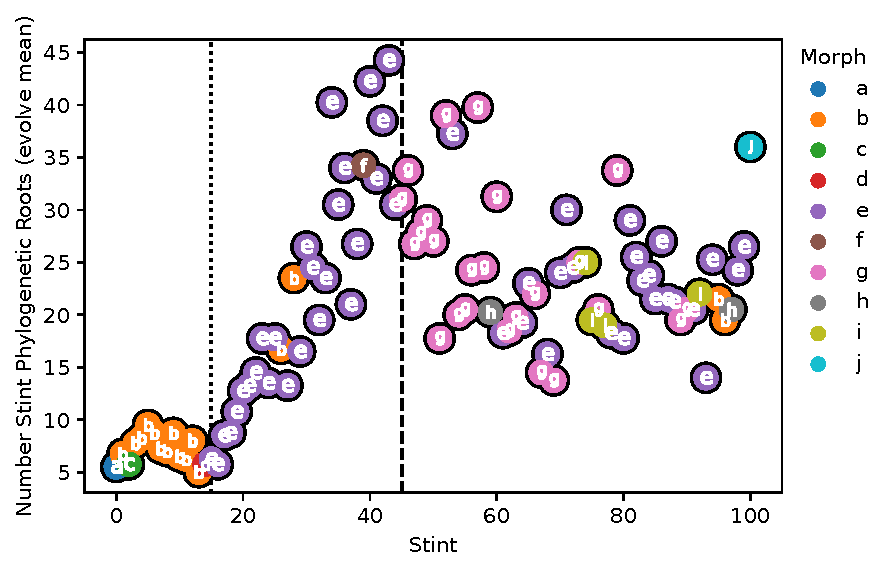
\includegraphics[width=\linewidth]{{plots/phylogeny/bucket=prq49+cat=morph+endeavor=16+transform=filter-Series-16005+viz=letterscatter-vline+x=stint+y=number-stint-phylogenetic-roots-evolve-mean+ext=}}

\caption{
Number of genomes from the beginning of a stint with extant offspring at the end of that stint. 
}
\label{fig:phylogeny:stint_roots}

\end{subfigure}%
\begin{subfigure}{0.5\textwidth}

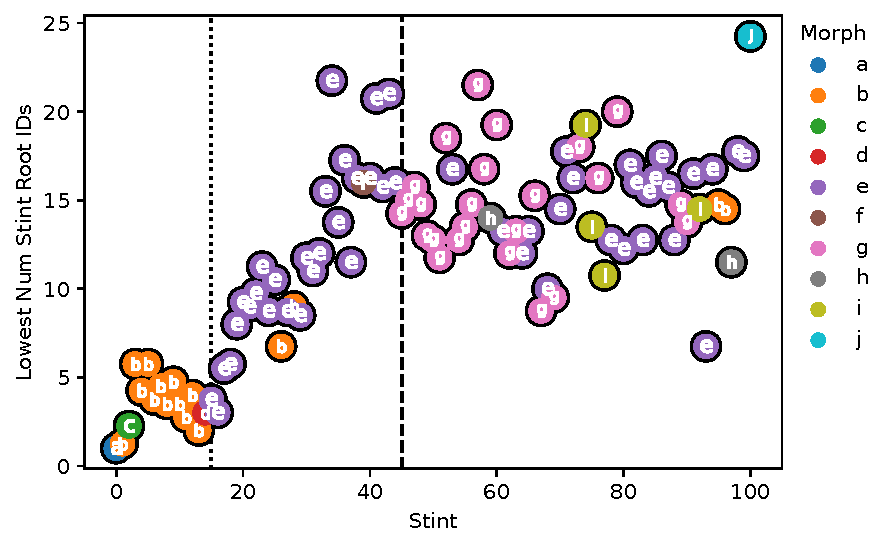
\includegraphics[width=\linewidth]{{plots/phylogeny/bucket=prq49+cat=morph+endeavor=16+transform=filter-Series-16005+viz=letterscatter-vline+x=stint+y=lowest-num-stint-root-ids+ext=}}

\caption{ Number of genomes with the lowest surviving original phylogenetic root ID from the beginning of a stint with extant offspring at the end of that stint.  }
\label{fig:phylogeny:lowestroot_stint_roots}

\end{subfigure}%
\begin{subfigure}{0.5\textwidth}

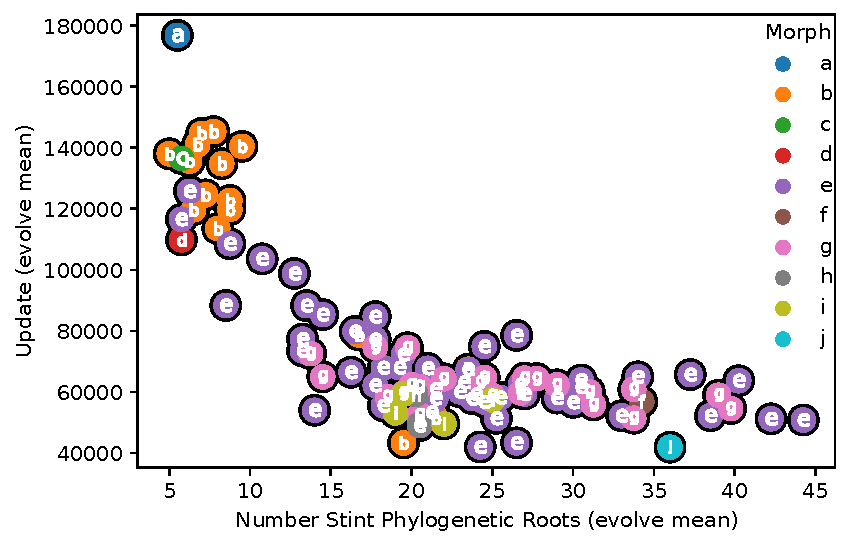
\includegraphics[width=\linewidth]{{plots/simulation/bucket=prq49+cat=morph+endeavor=16+transform=filter-Series-16005+viz=letterscatter+x=number-stint-phylogenetic-roots-evolve-mean+y=update-evolve-mean+ext=}}

\caption{
Relationship between number of simulation updates elapsed in a stint and the number of genomes seeded into a stint with extant descendants at the end of that stint.
}
\label{fig:phylogeny:updates_vs_stint_roots}

\end{subfigure}%

\begin{subfigure}{0.5\textwidth}

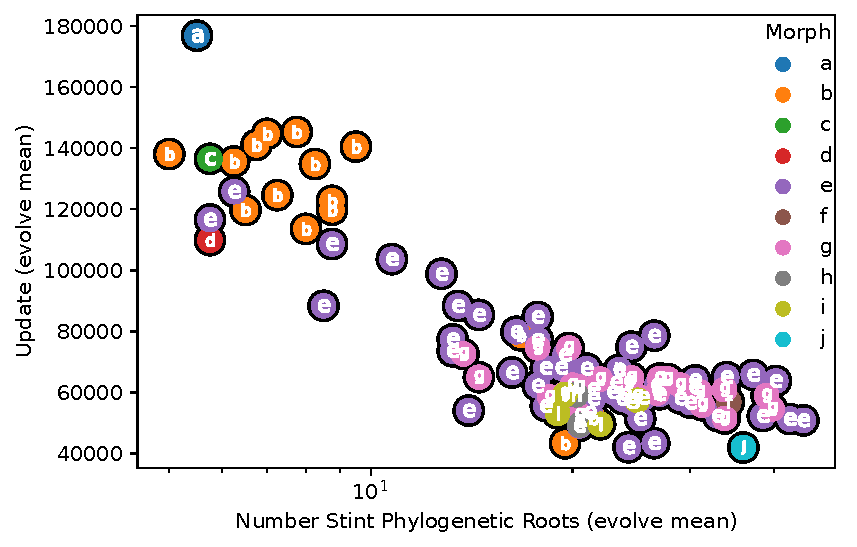
\includegraphics[width=\linewidth]{{plots/simulation/bucket=prq49+cat=morph+endeavor=16+transform=filter-Series-16005+viz=log-letterscatter+x=number-stint-phylogenetic-roots-evolve-mean+y=update-evolve-mean+ext=}}

\caption{ Relationship between number of simulation updates elapsed in a stint and the number of genomes seeded into a stint with extant descendants at the end of that stint, log axis. }
\label{fig:phylogeny:log_updates_vs_stint_roots}

\end{subfigure}%


\caption{
Phylogenetic statistics.
Color coding and letters correspond to qualitative morph codes described in Table \ref{tab:morph_descriptions}.
Dotted vertical line denotes emergence of morph $e$.
Dashed vertical line denotes emergence of morph $g$.
}
\label{fig:phylogeny}
\end{figure*}
